\documentclass[conference]{IEEEtran}
\IEEEoverridecommandlockouts
% The preceding line is only needed to identify funding in the first footnote. If that is unneeded, please comment it out.
\usepackage{cite}
\usepackage{amsmath,amssymb,amsfonts}
\usepackage{algorithmic}
\usepackage{graphicx}
\usepackage{textcomp}
\usepackage{lipsum}
\usepackage{xcolor}
% \usepackage{todonotes}
\usepackage{longtable}
\usepackage{float}
\usepackage{tikz}
\usepackage{pgfplots}
\usepgfplotslibrary{polar}


\def\BibTeX{{\rm B\kern-.05em{\sc i\kern-.025em b}\kern-.08em
    T\kern-.1667em\lower.7ex\hbox{E}\kern-.125emX}}
\begin{document}

\title{Analysis of Data Quality Management Maturity Level at PT Bank XYZ\\
% {\footnotesize \textsuperscript{*}Note: Sub-titles are not captured in Xplore and
% should not be used}
% \thanks{Identify applicable funding agency here. If none, delete this.}
}

\author{\IEEEauthorblockN{1\textsuperscript{st} Filzahanti Nuha Ramadhani}
\IEEEauthorblockA{
\textit{Fakultas Ilmu Komputer} \\
\textit{Universitas Indonesia}\\
Jakarta, Indonesia \\
filzahanti.nuha31@ui.ac.id}

\and
\IEEEauthorblockN{2\textsuperscript{rd} Jon Felix Germinian}
\IEEEauthorblockA{
\textit{Fakultas Ilmu Komputer} \\
\textit{Universitas Indonesia}\\
Jakarta, Indonesia \\
jon.felix@ui.ac.id}

\and
\IEEEauthorblockN{3\textsuperscript{nd} Samuel Mulatua Jeremy Nainggolan}
\IEEEauthorblockA{
\textit{Fakultas Ilmu Komputer} \\
\textit{Universitas Indonesia}\\
Jakarta, Indonesia \\
samuel.mulatua41@ui.ac.id}
}

\maketitle

\begin{abstract}
In the banking industry, high-quality data is essential for operational efficiency, regulatory compliance, and strategic decision-making. Understanding the maturity level of Data Quality Management (DQM) is crucial for PT Bank XYZ to identify gaps and uncover opportunities for improvement. Poor data quality can lead to significant risks, including inaccurate reporting, flawed decision-making, financial losses, and regulatory penalties. This study evaluates the DQM maturity at PT Bank XYZ using David Loshin’s Data Quality Framework and the Data Management Body of Knowledge (DMBOK) guidelines.

The research involves comprehensive interviews with key stakeholders to assess the bank's performance across eight DQM components, including governance, standards, and technology. The findings reveal an average maturity level of 2.04, classified as "Repeatable." While PT Bank XYZ demonstrates strength in data standard aspect, it struggles with deficiencies in data governance, quality protocols, and the implementation of advanced data technologies. These gaps hinder the bank’s ability to fully leverage its data assets for strategic growth and regulatory compliance.

To address these challenges, the study provides actionable recommendations aimed at enhancing DQM practices. By adopting these strategies, PT Bank XYZ can improve its data quality framework, reduce risks, and achieve a more sustainable competitive advantage.
\end{abstract}

\begin{IEEEkeywords}
data quality management; maturity model; maturity level; banking data
\end{IEEEkeywords}

\section{Introduction}
% Organizations today generate and manage data from a variety of sources, requiring robust systems to handle customer profiles, financial transactions, account management, and credit applications. Managing data quality (DQM) has become a critical focus for organizations, particularly in the banking sector, where accurate and reliable data serves as a cornerstone for operational efficiency and strategic growth. Poor data quality can lead to inaccuracies that hinder decision-making, such as selecting optimal business locations, and can expose organizations to reputational and financial risks.

% In the context of PT Bank XYZ, understanding the maturity level of Data Quality Management (DQM) is crucial to identify gaps and opportunities for improvement. The bank operates in a complex data ecosystem, integrating Core Banking Systems (CBS), Customer Relationship Management (CRM) platforms, and regulatory compliance tools. These systems demand high data quality to meet operational needs and comply with regulations, such as POJK No. 8/2023 on Anti-Money Laundering and Counter Terrorism Financing.

% To address these challenges, this paper explores the data quality maturity level of data quality management at PT XYZ and outlines strategies to enhance its governance framework. The study emphasizes the need for a holistic approach to data integration, quality monitoring, and regulatory compliance to ensure sustainable growth and resilience in the face of increasing data demands.

% The study is guided by the following research questions:
% \begin{enumerate}
%     \item What is the current maturity level of data quality management at PT XYZ?
%     \item How can PT XYZ improve its data quality management practices to address regulatory, operational, and strategic risks?
% \end{enumerate}

Organizations today generate and manage data from a variety of sources, requiring robust systems to handle customer profiles, financial transactions, account management, and credit applications. Managing data quality (DQM) has become a critical focus for organizations, particularly in the banking sector, where accurate and reliable data serves as a cornerstone for operational efficiency and strategic growth. Poor data quality can lead to inaccuracies that hinder decision-making, such as selecting optimal business locations, and can expose organizations to reputational and financial risks.

PT Bank XYZ, a microfinance-focused bank headquartered in Kabupaten Bandung Barat, operates a network of 24 branches and one cash office across Java, serving diverse customer needs through products like savings, deposits, and credit. As of October 2024, the bank manages assets of Rp 366 billion and employs approximately 300 staff, including an Information Technology (IT) division responsible for supporting business data analysis, regulatory reporting, and information systems. Despite its growth, the bank faces significant challenges, including fragmented data sources, increasing demands for internal and external data reporting, and frequent penalties from regulators such as OJK due to reporting errors. Additionally, regulatory requirements like POJK No. 8/2023 on Anti-Money Laundering and Counter-Terrorism Financing underscore the importance of accurate and up-to-date data management practices.

In the context of these challenges, understanding the maturity level of DQM at PT Bank XYZ is critical to identifying gaps and uncovering opportunities for improvement. The bank operates in a complex data ecosystem that integrates Core Banking Systems (CBS), Customer Relationship Management (CRM) platforms, and Loan Origination Systems (LOS), among others, without mechanisms for aggregating or monitoring data quality. As the organization strives to improve digital services and ensure compliance with evolving regulatory standards, addressing the risks of poor data quality—such as reputational damage, reporting errors, financial losses, and strategic missteps—becomes essential.

To address these challenges, this paper explores the maturity level of data quality management at PT Bank XYZ and outlines strategies to enhance its governance framework. The study emphasizes the need for a holistic approach to data integration, quality monitoring, and regulatory compliance to ensure sustainable growth and resilience in the face of increasing data demands. The objective of this study is to improve and evaluate the data quality management processes at PT Bank XYZ.

\section{Related Works}

This section explores three case studies highlighting diverse implementations of Data Quality Management (DQM) and Master Data Management (MDM). The first case study, as reported in \cite{dqmBPI2022}, focuses on PT BPI, where financial data quality management faces challenges due to errors, resulting in suboptimal decision-making in the public sector. The maturity level is at an initial stage, with reactive efforts managing structured financial data. The second case study, detailed in \cite{payani2023}, examines the National Remote Sensing Data Bank (BDPJN), which addresses the management of large volumes of satellite imagery data to support national planning. The organization demonstrates a maturity level ranging from defined to managed, handling unstructured remote sensing data. Lastly, \cite{hikmawati2021} discusses an MDM-based approach to improve data quality and governance, using the MD3M model to establish a "single source of truth" for transactional, inventory, and employee data. This study reflects a higher maturity level with a focus on consistent management of broader datasets, including customer, supplier, and material data. These case studies underscore the importance of tailored DQM and MDM practices to address organizational needs and data characteristics.


\section{Literature Review}

\subsection{Data Quality}

Data quality is essential for maintaining the usability, reliability, and trustworthiness of data. The Data Management Association International (DAMA) has identified six key dimensions of data quality that are widely acknowledged \cite{DAMA_2013} and applied across various fields \cite{wahyudi2023data, kiran2024addressing, antonio2024data}:  

\begin{itemize}
    \item \textbf{Completeness}: This dimension assesses whether all required data is present, ensuring no critical information is missing \cite{mahanti2019data}.
    \item \textbf{Uniqueness}: Ensures there is no redundant or duplicate data within a dataset, improving the overall integrity \cite{sebastiancoleman2022meeting}.
    \item \textbf{Timeliness}: Evaluates whether the data is up-to-date and relevant at the time of use, crucial for dynamic and real-time decision-making \cite{mashoufi2023data}.
    \item \textbf{Accuracy}: Measures whether the data accurately represents real-world values or concepts, ensuring trustworthiness \cite{west2021towards}.
    \item \textbf{Consistency}: Examines whether data values are aligned across multiple datasets or systems, preventing contradictions \cite{antonio2024data}.
\end{itemize}

These dimensions are foundational for establishing robust data governance and quality frameworks. For instance, studies such as \cite{wahyudi2023data} and \cite{kiran2024addressing} have demonstrated the application of these dimensions in various sectors, including healthcare, smart mobility, and financial institutions. Practical approaches to implementing these dimensions are also elaborated in works like \cite{sebastiancoleman2022meeting} and \cite{mahanti2019data}, making them essential for ensuring effective data management strategies.

\subsection{Data Quality Management}
Data quality management is a strategic approach aimed at preserving data quality by incorporating activities such as planning, execution, and control to assess and maintain high-quality data standards.

\subsubsection{Components of DQM}

DMBOK identifies critical components of DQM:
\begin{itemize}
    \item \textbf{Governance}: Establishing accountability structures for data quality.
    \item \textbf{Profiling and Cleansing}: Identifying and resolving quality issues.
    \item \textbf{Root Cause Analysis}: Addressing systemic issues that cause poor data quality.
    \item \textbf{Monitoring and Improvement}: Continuously assessing and enhancing quality metrics.
\end{itemize}

The DMBOK life cycle comprises six phases: planning, implementation, evaluation, monitoring, maintenance, and improvement. This iterative process ensures data quality aligns with organizational goals.

\subsubsection{Challenges in Data Quality Management}
DMBOK highlights several challenges:
\begin{itemize}
    \item \textbf{Data Silos}: Fragmented systems leading to inconsistent data.
    \item \textbf{Dynamic Data}: Increased volume and complexity in big data ecosystems.
    \item \textbf{Lack of Standards}: Disparate definitions of data quality across departments.
    \item \textbf{Human Error}: Manual interventions that introduce inaccuracies.
\end{itemize}


\subsection{Data Quality Maturity}

Managing data quality effectively requires aligning data quality practices with organizational activities \cite{loshin_dqi}. However, data management is often treated as secondary to functional needs, leading to siloed systems. A data quality maturity model, adapted from the Capability Maturity Model (CMM), helps organizations assess and improve their practices, moving from ad hoc processes to optimized systems.


\subsection{Data Quality Maturity Model}

The maturity model connects organizational data practices to higher levels of performance and quality by addressing key components of data management \cite{loshin_dqi}. 
% Organizational maturity in managing data quality is reflected in the following components:

% \begin{itemize}
%     \item \textbf{Data Quality Expectations}: Aligns understanding between IT and business to define and use data quality dimensions effectively.
%     \item \textbf{Policies}: Evolves from informal, undocumented approaches to fully integrated, auditable policies tied to business activities.
%     \item \textbf{Procedures}: High-performance organizations rely on well-defined processes and protocols to ensure information quality.
%     \item \textbf{Governance}: Develops through bottom-up information sharing and top-down formalization of responsibilities.
%     \item \textbf{Standards}: Maturity is reflected in how data standards are defined and implemented to ensure interoperability.
%     \item \textbf{Technology}: Shifts from tool acquisition to enterprise-wide, service-oriented approaches for data quality improvement.
%     \item \textbf{Performance Management}: Focuses on defining objectives, measuring conformance, and meeting performance goals.
% \end{itemize}


% First part of the table
\begin{table}[H]
\caption{Comparison of Maturity Models}
\label{tab:comparison-dqm-part1}
\centering
\begin{tabular}{|p{1.5cm}|p{3cm}|p{3cm}|}
\hline
\textbf{References} & \textbf{Maturity Levels} & \textbf{Dimensions} \\ \hline
Loshin \cite{loshin_dqi} & Initial, Repeatable, Defined, Managed, Optimized & Data Quality Expectations, Dimensions of Data Quality, Policies, Procedures, Governance, Standards, Technology, Performance Management \\ \hline
Ryu, K-S et al \cite{ryu2006dqm} & Initial, Defined, Managed, Optimized & Total corporate integration point of view, Data structure quality management point of view, Maturity stages point of view \\ \hline
Kirikoglu \cite{kirikoglu2017dqm} & Person, dependent and basic, Policies, standards, and procedures, Defined and stable, Managed and standardized, Continues improvement & Disciplined process, Standard consistent process, Predictable process, Continuously improving process \\ \hline
Ismael, C et al \cite{ismael2003caldea} & Initial, Definition, Integration, Quantitative Management, Optimizing & Data acquisition processes, Data product manufacturing process, and Data maintenance process \\ \hline
\end{tabular}
\end{table}

% % Second part of the table
% \begin{table}[h!]
% \caption{Comparison of Maturity Models (Part 2)}
% \label{tab:comparison-dqm-part2}
% \centering
% \begin{tabular}{|p{1.5cm}|p{3cm}|p{3cm}|}
% \hline
% \textbf{References} & \textbf{Maturity Levels} & \textbf{Dimensions} \\ \hline

% \end{tabular}
% \end{table}

In this study, the author selected David Loshin's data quality maturity model. This model was chosen because its dimensions are comprehensive and more adaptable for application in various companies, including PT Bank XYZ, compared to other models.

% \section{Research Method}

% This research stage as shown by figure \ref{fig:research-step} begins with problem identification by asking Director of Operations where the key issue is defined to guide the study. Next, a literature review is conducted to previous research on the topic. Following this, a research instrument is developed using Data Quality Framework by David Loshin \cite{loshin_dqi} as interview guides. After the data is collected, a data quality management maturity assessment is performed. Finally, based on the findings, a data quality improvement strategy is developed to enhance the quality and effectiveness of the data for future analysis based on the Data Quality Activities by DMBOK.
% \begin{figure}[H]
% \centerline{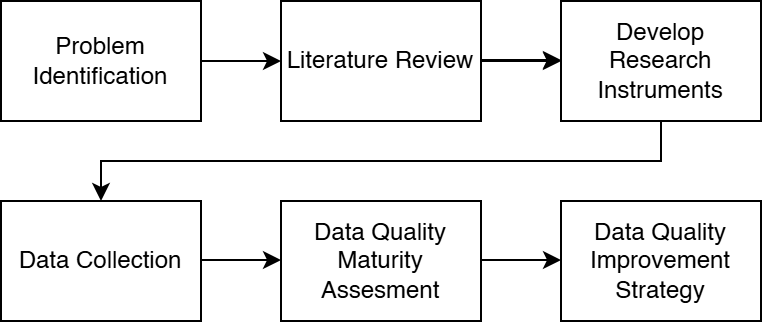
\includegraphics[width=0.4\textwidth]{figures/AlurPenelitian.png}}
% \caption{Research Stages}
% \label{fig:research-step}
% \end{figure}

% \subsection{Research Instruments}

% In this study, the DQM maturity level characteristic matrix, derived from David Loshin’s Data Quality Framework (DQF) \cite{loshin_dqi} is used as the instrument. The matrix consists of a checklist containing 121 characteristics spread across 8 components defined in the DQF, as summarized in TABLE \ref{tab:questionnare-areas}. 
% \begin{table}[H]
% \caption{Table of Questionnaire Areas and Number of Questions}
% \label{tab:questionnare-areas}
% \centering
% \begin{tabular}{|l|c|}
% \hline
% \textbf{Questionnaire Area} & \textbf{\#Question} \\
% \hline
% Data Quality Expectations & 18 \\
% \hline
% Data Quality Dimensions & 14 \\
% \hline
% Information Policies & 17 \\
% \hline
% Data Quality Protocols & 20 \\
% \hline
% Data Governance & 18 \\
% \hline
% Data Standards & 20 \\
% \hline
% Data Quality Technology & 12 \\
% \hline
% Performance Management & 14 \\
% \hline
% \textbf{Total} & \textbf{133} \\
% \hline
% \end{tabular}
% \end{table}

% \subsection{Data Collection}
% Data was collected through interviews with two Subject Matter Experts (SME) in the organization, Head of Information Technology (IT) and Head of Operations. The interviews included a set of pre-planned questions using the research instrument to understand how the organization manages data quality. Interviews were conducted in person or online to accommodate participants’ schedules. The responses were recorded and transcribed for analysis.

% \subsection{Data Analysis Techniques for Assessing Data Quality Maturity Levels}
% This research used a mixed-methods approach for data analysis combining both qualitative and quantitative methods. Data was collected through interviews using preplanned questions. The interviews were transcribed for analysis and the transcripts were reviewed to evaluate the characteristics of each component in the DQF. \cite{loshin_dqi}.
% Each characteristic was assessed and given a score 1 if it was true and 0 if it was not. The scores for each level within a component were averaged and summed to find the overall quality of the component. The overall data quality maturity level was then calculated by averaging the maturity levels of each component.

% \subsection{Data Quality Improvement Strategy}
% The characteristics that the organization has not fully met are identified. These characteristics are marked by a score of 0 in the evaluation. They highlight areas where the organization’s data quality management practices need improvement. These characteristics are mapped to the Data Quality Management (DQM) activities in the DMBOK \cite{DAMA_2013}. This mapping helps align the organization’s practices with established best practices. From this, the analysis provides specific recommendations and strategies to improve data quality management. 


\section{Research Methodology}

This study adopts a structured approach to evaluate and improve the data quality management (DQM) maturity level at PT Bank XYZ. The methodology integrates qualitative and quantitative methods, using David Loshin’s Data Quality Framework (DQF) and the Data Management Body of Knowledge (DMBOK) as guiding models. Figure \ref{fig:research-stages} provides an overview of the research stages, while the subsequent subsections outline the specific methods employed.

\subsection{Research Stages}

The research process consists of the following stages (illustrated in Fig. \ref{fig:research-stages}):
\begin{itemize}
    \item \textbf{Problem Identification:} Discussions with the Director of Operations were conducted to pinpoint key organizational challenges related to data quality management.
    \item \textbf{Literature Review:} Relevant studies and frameworks on DQM and maturity assessment were reviewed to establish a theoretical foundation.
    \item \textbf{Research Instrument Development:} A customized checklist was designed using Loshin’s DQM framework to assess maturity across eight components.
    \item \textbf{Data Collection:} Qualitative data was gathered through stakeholder interviews, targeting subject matter experts (SMEs) within the organization.
    \item \textbf{Data Analysis and Assessment:} The collected data was evaluated to calculate the organization’s DQM maturity level.
    \item \textbf{Strategy Development:} Recommendations were proposed based on the gaps identified in the maturity assessment, aligning with DMBOK best practices.
\end{itemize}

\begin{figure}[h]
\centerline{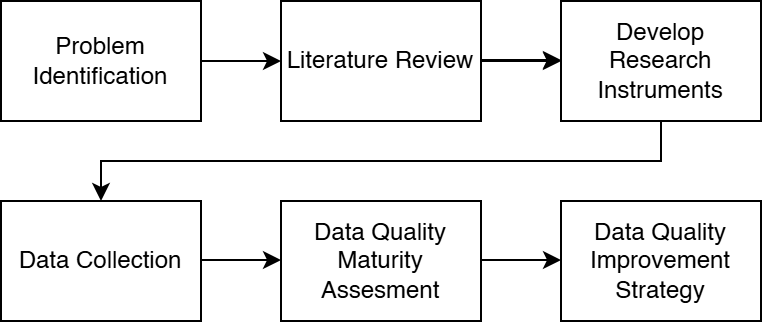
\includegraphics[width=0.45\textwidth]{figures/AlurPenelitian.png}}
\caption{Research Stages}
\label{fig:research-stages}
\end{figure}

\subsection{Research Instrument}

The primary tool for data collection was the DQM Maturity Level Characteristic Matrix, derived from David Loshin’s DQM Framework \cite{loshin_dqi}. The matrix includes a checklist of 133 characteristics across eight DQM components, as summarized in Table \ref{tab:questionnaire}. These components cover key areas such as governance, standards, and performance management, ensuring a comprehensive evaluation of the organization’s data quality practices.

\begin{table}[h]
\caption{Questionnaire Areas and Number of Questions}
\label{tab:questionnaire}
\centering
\begin{tabular}{|l|c|}
\hline
\textbf{Questionnaire Area} & \textbf{Number of Questions} \\
\hline
Data Quality Expectations & 18 \\
Data Quality Dimensions & 14 \\
Information Policies & 17 \\
Data Quality Protocols & 20 \\
Data Governance & 18 \\
Data Standards & 20 \\
Data Quality Technology & 12 \\
Performance Management & 14 \\
\hline
\textbf{Total} & \textbf{133} \\
\hline
\end{tabular}
\end{table}

\subsection{Data Collection}

Data collection focused on qualitative insights gathered through structured interviews with two Subject Matter Experts (SMEs): the Head of Information Technology (IT) and the Head of Operations. The interviews were guided by pre-designed questions derived from the DQM checklist to explore organizational practices in data management. Interviews were conducted both in-person and virtually, ensuring flexibility in scheduling. All responses were recorded, transcribed, and organized for subsequent analysis.

Although interviews were the primary method, incorporating surveys or benchmarking against similar organizations could have added more comparative insights. Future studies should consider these additional methods to enhance robustness.

\subsection{Data Analysis}

A structured scoring rubric was used to evaluate the collected data.

\begin{itemize}
    \item \textbf{Scoring Mechanism:} Each characteristic in the DQM framework was evaluated and assigned a score:
    \begin{itemize}
        \item \textbf{1:} If the characteristic was fully met.
        \item \textbf{0:} If the characteristic was not met.
    \end{itemize}
    \item \textbf{Component-Level Averages:} Scores within each DQM component were averaged to compute a maturity level for that component.
    \item \textbf{Overall Maturity Level:} An overall maturity score was calculated by averaging the maturity levels across all components.
\end{itemize}


\subsection{Development of Improvement Strategy}

The analysis identified specific characteristics that were not met (scored 0), highlighting gaps in the organization’s DQM practices. These gaps were mapped to actionable strategies based on \cite{loshin_dqi} data quality management maturity model. For each gap, tailored recommendations were proposed to improve data governance, technology, and overall maturity.

To ensure the feasibility and sustainability of improvements, the strategy targets achieving one maturity level above the organization’s current level \cite{loshin_dqi}. While organizations may aspire to reach the highest levels of maturity, attempting to make such a significant leap can overwhelm resources and disrupt ongoing processes. A gradual approach, focusing on advancing one level at a time, is more practical and aligns with the organization’s operational capacity. This incremental improvement allows PT Bank XYZ to consolidate its gains at each stage, ensuring that new processes, policies, and technologies are effectively integrated before pursuing further advancements.

\section{Result and Discussions}
\subsection{Assessment Result}
The results indicated that three areas met the initial level, four areas were at the repeatable level, and one reached the defined level. As a result, the overall average maturity level was 2.04. Table \ref{tab:maturity-level} provides more details on the expected level for each area.

\begin{table}[H]
\caption{Maturity Level}
\label{tab:maturity-level}
\centering
\begin{tabular}{|p{0.3cm}|p{3cm}|p{1cm}|p{2cm}|}
\hline
\textbf{No} & \textbf{Questionnaire Area} & \textbf{Maturity Level}&\textbf{Level Description} \\
\hline
1 & Data Quality Expectations & 2.08 & Repeatable\\
\hline
2 & Data Quality Dimensions & 2.00 & Repeatable\\
\hline
3 & Information Policies & 1.90 & Initial\\
\hline
4 & Data Quality Protocols & 2.33 & Repeatable \\
\hline
5 & Data Governance & 1.33 & Initial \\
\hline
6 & Data Standards & 3.00 & Managed \\
\hline
7 & Data Quality Technology & 1.58 & Initial\\
\hline
8 & Performance Management & 2.08 & Repeatable\\
\hline
\multicolumn{2}{|l|}{\textbf{Average}} & \textbf{2.04}& \textbf{Repeatable} \\
\hline
\end{tabular}
\end{table}

Based on the interviews, the current condition of each data quality component in the company is as follows.
\begin{itemize}
\item \textbf{Data Quality Expectations}: This organization lacks internal documents outlining data quality expectations and relies only on related regulations like Peraturan Otoritas Jasa Keuangan (POJK) and Surat Edaran Otoritas Jasa Keuangan (SEOJK). There are no clear expectations or documentation for data quality dimensions.
\item \textbf{Data Quality Dimensions}: The company has no formal definition of data quality or clear categories for measuring it. There are no rules or reports for data quality, and no connection between data quality and business impacts. There is no data quality matrix, SLA document, or monitoring of SLA.
\item \textbf{Information Policy}: The company has no formal data quality policy or guidelines for handling data issues. The existing SLA between Pusintek and Biro SDM does not address data quality, and there is no automated system for data quality governance.
\item \textbf{Data Quality Protocols}:The company has identified some causes of data quality issues, but errors keep repeating. Root cause analysis is done case by case without using data quality or validation rules. There is no procedure to check data accuracy or validity. There is also no process for handling incomplete or incorrect data.
\item \textbf{Data Governance}: The company does not have a dedicated data steward, and data management responsibilities are handled by the IT division. There is no team or manager for data repairs, and no group exists to design or recommend data governance programs and policies. There are also no guiding principles or data governance policies in place.
\item \textbf{Data Standards}: There are no defined data elements to identify information, and no certification activities for trusted or owned data sources. Metadata standards are still controlled by IT and there is no process to manage data exchange standards. Also, there is no board to oversee and maintain internal and external data standards.
\item \textbf{Data Quality Technology}: The company lacks tools to objectively measure data quality, find or connect data, and there is no standard procedure for using data quality technology to assess or improve it. Additionally, validation processes based on business rules have not been implemented.
\item \textbf{Performance Management}: The company does not use data profiling to identify errors, lacks a framework to analyze the impact of data quality, and has no defined data quality service components to detect errors early in the process.
\end{itemize}


A good practice in data quality management is to set the target maturity level one level above the current state as shown in Table \ref{tab:target-maturity-level}. Although organizations might want to reach the highest level of maturity, the challenges they face and the advisory role of data quality managers often make this difficult. Instead, it is better to reach for a level that meets the organization's goals while still being achievable within the team’s capabilities \cite{loshin_dqi}. Figure \ref{fig:maturity-level-spider-graph} shows the assessment result of PT Bank XYZ

\begin{table}[H]
\caption{Target Maturity Level}
\label{tab:target-maturity-level}
\centering
\begin{tabular}{|p{0.3cm}|p{3cm}|p{1cm}|p{2cm}|}
\hline
\textbf{No} & \textbf{Questionnaire Area} & \textbf{Target Maturity Level}&\textbf{Level Description} \\
\hline
1 & Data Quality Expectations & 3 & Defined\\
\hline
2 & Data Quality Dimensions & 3 & Defined\\
\hline
3 & Information Policies & 2 & Repeatable\\
\hline
4 & Data Quality Protocols & 3 & Defined \\
\hline
5 & Data Governance & 2 & Repeatable \\
\hline
6 & Data Standards & 4 & Managed \\
\hline
7 & Data Quality Technology & 2 & Repeatable\\
\hline
8 & Performance Management & 3 & Defined\\
\hline
\end{tabular}
\end{table}

By targeting a level just above the current one, organizations can make gradual improvements without overwhelming the staff. This approach helps achieve data quality benefits step by step, with clear goals along the way. In the end, this method leads to more manageable and effective improvements in data quality \cite{loshin_dqi}.

% \begin{figure}[H]
%     \centering
%     \begin{tikzpicture}[scale=0.3]
%         % Define the origin of the spider graph
%         \coordinate (origin) at (0, 0);

%         % Define the maturity levels and corresponding labels
%         \foreach[count=\i] \radius/\label in {
%             2.08/Data Quality \\ Expectations,
%             2.00/Data Quality \\ Dimensions,
%             1.90/Information \\ Policies,
%             2.33/Data Quality \\ Protocols,
%             1.33/Data \\ Governance,
%             3.00/Data \\ Standards,
%             1.58/Data Quality \\ Technology,
%             2.08/Performance \\ Management}{
%             \coordinate (\i) at (\i * 360 / 8: \radius * 3); % Scale radius by 3 for better visibility
%             \node[align=center] (label) at (\i * 360 / 8: 11) {\normalsize\label}; % Place labels
%             \draw[gray, dotted] (origin) -- (label); % Connect labels to the origin
%         }

%         % Draw the filled polygon connecting all points
%         \draw [fill=blue!20, opacity=.7] (1)
%                                     \foreach \i in {2,...,8}{-- (\i)} -- cycle;

%         % Add the grid lines for reference
%         \foreach \r in {1, 2, 3} {
%             \draw [gray, dotted] (0, 0) circle (\r * 3);
%         }

%         % Add concentric circle labels
%         % \node at (0, 0) {\footnotesize\textbf{0}};
%         \node at (112.5:3) {\footnotesize\textbf{1}};
%         \node at (112.5:6) {\footnotesize\textbf{2}};
%         \node at (112.5:9) {\footnotesize\textbf{3}};
%     \end{tikzpicture}
%     \caption{Maturity Level Spider Graph}
%     \label{fig:maturity-level-spider-graph}
% \end{figure}

\begin{figure}[H]
    \centering
    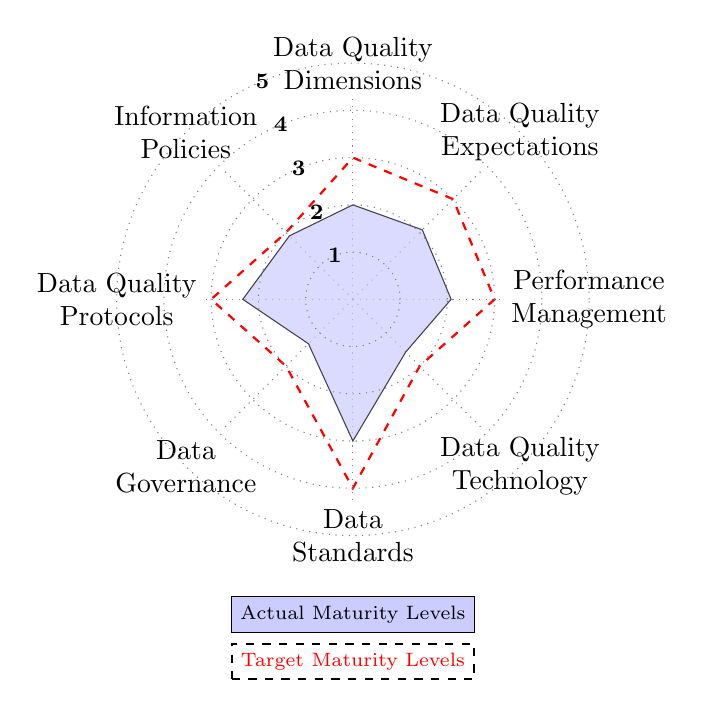
\begin{tikzpicture}[scale=0.2]
        % Define the origin of the spider graph
        \coordinate (origin) at (0, 0);

        % Define the actual maturity levels and corresponding labels
        \foreach[count=\i] \radius/\label in {
            2.08/Data Quality \\ Expectations,
            2.00/Data Quality \\ Dimensions,
            1.90/Information \\ Policies,
            2.33/Data Quality \\ Protocols,
            1.33/Data \\ Governance,
            3.00/Data \\ Standards,
            1.58/Data Quality \\ Technology,
            2.08/Performance \\ Management}{
            \coordinate (actual-\i) at (\i * 360 / 8: \radius * 3); % Scale radius by 3 for better visibility
            \node[align=center] (label) at (\i * 360 / 8: 15) {\normalsize\label}; % Place labels at level 5
            \draw[gray, dotted] (origin) -- (label); % Connect labels to the origin
        }

        % Define the target maturity levels
        \foreach[count=\i] \radius in {
            3, % Data Quality Expectations
            3, % Data Quality Dimensions
            2, % Information Policies
            3, % Data Quality Protocols
            2, % Data Governance
            4, % Data Standards
            2, % Data Quality Technology
            3  % Performance Management
        }{
            \coordinate (target-\i) at (\i * 360 / 8: \radius * 3); % Scale radius by 3 for better visibility
        }

        % Draw the actual maturity level polygon
        \draw [fill=blue!20, opacity=.7] (actual-1)
                                    \foreach \i in {2,...,8}{-- (actual-\i)} -- cycle;

        % Draw the target maturity level polygon
        \draw [red, thick, dashed] (target-1)
                                    \foreach \i in {2,...,8}{-- (target-\i)} -- cycle;

        % Add the grid lines for reference
        \foreach \r in {1, 2, 3, 4, 5} {
            \draw [gray, dotted] (0, 0) circle (\r * 3);
        }

        % Add concentric circle labels
        \node at (112.5:3) {\footnotesize\textbf{1}};
        \node at (112.5:6) {\footnotesize\textbf{2}};
        \node at (112.5:9) {\footnotesize\textbf{3}};
        \node at (112.5:12) {\footnotesize\textbf{4}};
        \node at (112.5:15) {\footnotesize\textbf{5}};

        % Add legend at the bottom
        \node[fill=blue!20, draw=black, align=center] at (0, -20) {\scriptsize Actual Maturity Levels};
        \node[red, thick, dashed, draw=black, align=center] at (0, -23) {\scriptsize Target Maturity Levels};
    \end{tikzpicture}
    \caption{Maturity Level Spider Graph with Target Levels}
    \label{fig:maturity-level-spider-graph}
\end{figure}


\subsection{Recommendations}
% Gaps between the company current data quality and the target expectations through assessments or interviews is identified. These gaps show characteristics that are not yet implemented. Based on these gaps, recommendations are made to improve DQM using DQM activities from the DMBOK to reach one level above the current state. The complete gap analysis to gap analysis can be seen in Table \ref{tab:mapping}.
% The activities to improve Data Quality Management (DQM) based on the mapping to the Data Management Body of Knowledge (DMBOK) are listed below:
% \begin{enumerate}
%     \item Manage Data Quality Rules (DQM Activity 7.1) \\ Managing data quality rules means analyzing data to create rules, adding rules to system processes, and documenting them clearly. The rules should support business goals, be checked through data analysis, and confirmed by experts. They should also be available to all data users for better understanding and feedback. Below is a list of characteristics the company has not yet implemented, based on component maturity description of data quality management by David Loshin \cite{loshin_dqi}.
%         \begin{itemize}
%             \item "No data quality expectations have been documented"
%             \item "Expectations associated with dimensions of data quality associated with data values, formats, and semantics can be articulated using data quality rules
%             \item "Policies are informal"
%         \end{itemize}
% \end{enumerate}

The assessment results highlighted several gaps between the company’s current data quality management (DQM) practices and the target expectations. These gaps represent characteristics that have not yet been implemented and hinder the organization’s progress toward higher maturity levels. Recommendations are presented below, prioritized to ensure a logical sequence of improvements that align with business goals and operational feasibility. The detailed mapping of gaps and recommended activities to the Data Management Body of Knowledge (DMBOK) is provided in Table \ref{tab:mapping}.

\begin{table*}[hbt!]
\caption{Mapping the gaps in DQM maturity levels to the activities outlined in DQM-DMBOK}
\label{tab:mapping}
\centering
\begin{tabular}{|p{2cm}|p{5cm}|p{5cm}|p{2cm}|}
\hline
\textbf{Data Quality Component} & \textbf{Characteristics} & \textbf{Recommendations} & \textbf{DMBOK Activity} \\
\hline
Data Quality Expectations (target = 3) & "No data quality expectations have been documented", "Expectations associated with dimensions of data quality associated with data values, formats, and semantics can be articulated using data quality rules" & The company should consider create internal documents for data quality expectations, consistently document rules, define them by quality aspects, and connect them to business impact for better results. The company should include expectations and guidelines for data quality dimensions, such as data values, to help clearly define what is being measured and improve consistency in measurement and issue management & 7.1 \\

\hline
Data Quality Dimensions (target = 3) & "Recognition of common dimensions for measuring quality of data values", "Basic reporting for simple data quality measurements" & It is recommended that the company define data quality and establish common dimensions for measuring data values. This will help track data quality, inform users, and manage risks from changes. The company should create reports on data quality, including a scorecard, trends, SLA metrics, and issue tracking, to show progress and the impact of improvements. & 7.2, 7.5 \\
\hline
Information Policies (target = 2) & "Policies are informal", "Policies are undocumented", "Initial policies defined for reacting to data issues" & The company is encouraged to create a formal data quality policy, document clear data quality rules, and integrate them into system development. This will set expectations, ensure control, and support ongoing measurement and reporting & 7.1 \\
\hline
% Information Policies (target = 2) & " Initial policies defined for reacting to data issues" & There is no policy for handling data issues & 7.1 \\
% \hline
Data Quality Protocols (target = 3) &
% "Failures reacted to reactively, with no coordination with business processes."
"Root causes unidentified, errors repeated", 
"Errors tracked for incompleteness and invalid syntax", 
"Basic root cause analysis via data quality rules"
& 
There is a need for data controls to be deployed across the enterprise, participants to publish data quality measurements, and data quality management practices to be transparent.
& 7.4\\
\hline
Data Governance (target = 2)& 
"Informal communication about data quality between IT and other divisions", 
% "IT support handles most data quality issues without a formal strategy."
"No dedicated data stewardship; responsibilities are ad hoc", 
"Best practices for data quality are shared informally"
% "No formal workgroup for data governance or guiding principles in development."
&
There is a need to formalize Data Stewardship roles and responsibilities, develop and document guiding principles, data quality charter, and policies, establish a formal data governance workgroup with key stakeholders.
& 7.5 \\
\hline
Data Standards (target = 4) & 
"Certification process for trusted data sources is still not defined", 
% "Master data reference sets have been identified and are managed, but further formalization is needed."
"No formal process for overseeing the management of exchange standards", 
"No Data Standards Oversight Board exists"
& 
There is a need to implement a Master Data Management (MDM) solution to formalize master data concepts and develop a clear taxonomy for data standards, ensuring it is endorsed and widely adopted.
& 7.3 \\
\hline
Data Quality Technology (target = 2) & 
"Tools for assessing objective data quality not available", 
"Data parsing, standardization, and cleansing available", 
"Data quality technology for matching and linking not available"
& 
There is a need to implement tools for assessing data quality, establish technology for data matching, define standardized procedures for quality assessment, and use business rule-based validation techniques.
% "Standardize technology components for data validation, certification, assurance, and reporting across the organization."
% "Ensure technology components are standardized at both the service and implementation layers."
& 7.2 \\

\hline
Performance Management (target = 3) & "Data profiling used to identify data failures in process" & It is advisable for the company to implement data profiling to identify errors, set clear data quality expectations, establish system controls, and support ongoing measurement and reporting. & 7.1 \\
\hline
\multicolumn{2}{|l|}{\textbf{Average}} & \textbf{2.04} & \textbf{Repeatable} \\
\hline
\end{tabular}
\end{table*}



The first recommendation is to formalize data quality rules as this serves as the foundation for consistent data quality practices. The organization should develop and document formal data quality expectations and policies while defining rules associated with data values, formats, and semantics to ensure alignment with business objectives. These rules must be disseminated to all data users to promote awareness and encourage compliance. Achieving 100% documentation coverage of these rules within six months is suggested as a measurable target.

The second recommendation focuses on strengthening the data governance framework, which is essential for assigning accountability and ensuring sustained improvements. Establishing a formal data stewardship role or team responsible for data quality management is critical, alongside creating guiding principles, a data quality charter, and governance policies. A cross-functional governance workgroup should also be formed to oversee data quality initiatives. The organization should aim to establish this governance framework and approve the related policies within three months.

Implementing data quality technology is the third recommendation. Advanced tools for data quality assessment and validation are necessary to automate processes and ensure real-time monitoring. Deploying tools for data profiling, validation, and cleansing, as well as introducing rule-based validation techniques to detect errors in real-time, will significantly improve operational efficiency. Additionally, technology that matches and links data across systems should be adopted. A 50% reduction in data errors through automated validation tools within 12 months is a key goal for this initiative.

Lastly, improving performance management is essential to establish mechanisms for measuring, monitoring, and reporting data quality effectively. Key metrics such as data error rates, SLA adherence, and improvement trends should be defined and integrated into a data quality scorecard for regular internal and external reporting. These metrics should also be incorporated into the organization’s performance review process. Implementing these scorecards within six months and reporting monthly trends will help track progress and ensure accountability.

\subsubsection{Measurable Goals and Roadmap}

In the short term, the organization should focus on formalizing data quality rules and disseminating them across the organization. Additionally, establishing a dedicated data governance team and approving guiding policies are critical initial steps. These efforts will lay the groundwork for subsequent improvements.

In the long term, deploying data quality tools and automating validation processes are key priorities. These efforts should be complemented by integrating data quality metrics into performance reviews and achieving targeted reductions in error rates. This phased approach ensures manageable progress and aligns with the organization’s capacity for change.



\section{Conclusions and Future Works}

\subsection{Conclusions}

The study's findings lead to the following conclusions:

\begin{enumerate}
    \item The results of measuring the maturity level at PT Bank XYZ using the Loshin and DMBOK method \cite{loshin_dqi}\cite{DAMA_2013} indicate that the organization is still at level two(Repeatable). Our study shows that PT Bank XYZ has good level of Data Standard but is lacking in other areas such as Data Quality Technology and Data Governance.
    \item PT Bank XYZ has demonstrated a varying level of maturity across different data management domains. While the organization excels in data standards, achieving a maturity level of 3.00 (Managed), there is still significant room for improvement in areas such as Data Governance (1.33, Initial), Information Policies (1.90, Initial), and Data Quality Technology (1.58, Initial). The maturity levels for Data Quality Expectations, Data Quality Dimensions, and Data Quality Protocols fall within the Repeatable stage, indicating a developing but inconsistent approach. To advance towards higher maturity, the bank should focus on formalizing data governance structures, improving technological support for data quality, and establishing clearer policies and protocols for managing data.
    \item The Loshin Data Quality Management (DQM) framework helps assess an organization's data quality practices and maturity. It identifies gaps across key dimensions like governance, technology, and performance management, offering actionable recommendations for improvement. PT Bank XYZ can use this framework to enhance data management, strengthen governance, and ensure more reliable data.
\end{enumerate}


\subsection{Limitations and Future works}

The author hopes that this research can benefit PT Bank XYZ. Based on the recommendations from the research results, PT Bank XYZ can plan and prepare to implement the given recommendations. Thus, it is expected that data quality management at PT Bank XYZ can be implemented and improved, leading to better data quality. The author also hopes this research will be useful for future studies. The following are the author's suggestions for future research: 
\begin{enumerate}
    \item Further evaluation can be conducted using the same method. It is within a organization's interest to reach a higher data quality management maturity level.
    \item Maturity measurement must be carried out continuously to reach the final level.
\end{enumerate}


\section*{ACKNOWLEDGMENT}


Hopefully this research will provide value and benefit to readers, despite any shortcomings in its writing. The author extends gratitude to everyone who has offered support and assistance in completing this paper.

\section*{Work Division}
\begin{itemize}
    \item Samuel: Data collection, Conducting Interview, Abstract, Introduction, topic, Process the data using Excel
    \item Jon: Literature Study, State of the art, Result Discussion, Conclusion (Assessment Result, Gap Analysis), \LaTeX{} Formatting
    \item Filza: Research Method, Result and Discussion (Assessment Result, Gap Analysis)
\end{itemize}





% \section*{References}
\bibliographystyle{IEEEtran}
\bibliography{references}

\end{document}
